\documentclass[12pt,a4paper]{article}
\usepackage[utf8]{inputenc}
\usepackage[margin=1.5cm]{geometry}
\usepackage{amsmath}
\usepackage{amssymb}
\usepackage{amsthm} 
\usepackage{graphicx}
\usepackage{mathtools}

\DeclarePairedDelimiter{\abs}{\lvert}{\rvert}
\newcommand{\inter}{\begin{matrix}\prod\end{matrix}}
 
\begin{document}
\section*{LEZIONE 16}
\subsection*{Integrazione numerica (formula quadratica): stabilità dell'operatore di integrazione, formule di quadratura algebriche e composte, convergenza e stabilità, formule a pesi positivi}

Dopo aver discusso alcune tecniche per l'approssimazione di funzioni da dati discreti, in questo capitolo ci occuperemo dell'approssimazione di operazioni funzionali (spesso chiamate operatori) sempre a partire da un campionamento finito, in particolare studieremo il calcolo approssimato di integrali definiti ("integrazione numerica") e il calcolo approssimato di derivate ("derivazione numerica").\\
In questa lezione introdurremo i metodi di calcolo di integrali basati su opportune somme pesate, le cosiddette "formule di quadratura".\\
La prima cosa da osservare è che l'operatore di integrazione di $f\in C[a,b]$
\begin{equation*}
    I:f\longmapsto I(f)=\int_a^bf(x) dx\  \  \  \in\mathbb{R}
\end{equation*}
è stabile, nel senso che controllando gli errori su $f$ si controllano gli errori su $I(f)$.\\ Infatti se $\tilde{f}\approx f$ con 
\begin{equation*}
dist(f,\tilde{f})= \max_{x\in[a,b]}\abs{f(x)-\tilde{f}(x)}\leq\varepsilon
\end{equation*}
allora
\begin{equation*}
\begin{split}
        \abs*{I(f)-I(\tilde{f})} & = \abs*{\int_a^b f(x)dx-\int_a^b \tilde{f}(x)dx} \\
        & = \abs*{\int_a^b(f(x)-\tilde{f}(x))dx} \\
        & = \abs*{I(f-\tilde{f})} \\
        & \leq \int_a^b \abs*{f(x)-\tilde{f}(x)}dx \\
        & = I\left(\abs*{f-\tilde{f}}\right) \\
        & \leq \int_a^b dist(f,\tilde{f})dx \\
        & = dist(f, \tilde{f})\int_a^b 1 dx \\
        & = dist(f, \tilde{f})(b-a)\\
        & \leq\varepsilon(b-a)
\end{split}
\end{equation*}
dove abbiamo usato la linearità dell'operatore di integrazione
\begin{equation*}
        I(\alpha f+\beta g)=\alpha I(f)+\beta I(g)\quad \forall f,g\in C[a,b],\quad \alpha,\beta\in\mathbb{R}
\end{equation*}
e la disuguaglianza fondamentale
\begin{equation*}
    \abs*{I(f)} \leq I(\abs*{f})
\end{equation*}
Quindi abbiamo a che fare con un \underline{"problema stabile"} perchè "errori (sufficientemente) piccoli sulla funzione portano ad errori piccoli sul valore dell'integrale".\\
Ricordiamo che questo della \underline{stabilità del problema} è un concetto "a monte" della soluzione con algoritmi approssimati, che andranno cercati in modo che siano convergenti e stabili. \\Ben diversa è la situazione con l'operatore di derivazione, dove scopriremo che ci sono "funzioni arbitrariamente vicine con derivate arbitrariamente distanti", cioè un'instabilità intrinseca del problema che verrà ereditata dagli algoritmi risolutivi (che non potranno mai essere veramente stabili).\\ Esemplifichiamo  qui sotto questi concetti con alcuni disegni 
\newline \newline
\textbf{STABILITÀ DELL'INTEGRALE}
\begin{center}
    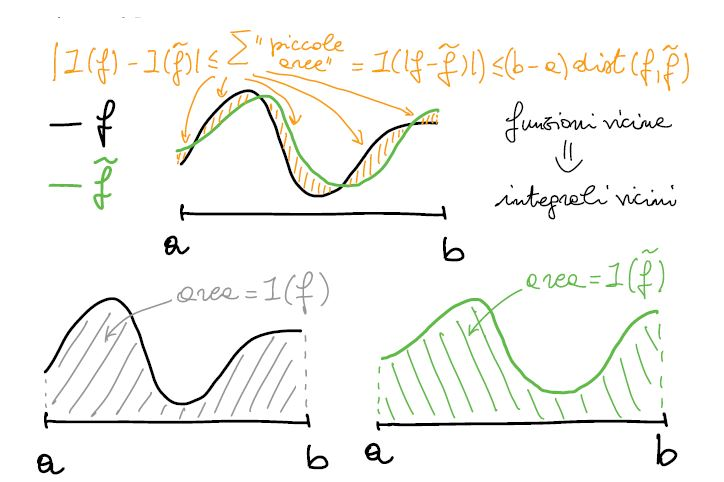
\includegraphics[scale=0.6]{calcolo5.JPG}
\end{center}
\textbf{INSTABILITÀ DELLA DERIVATA}
\begin{center}
    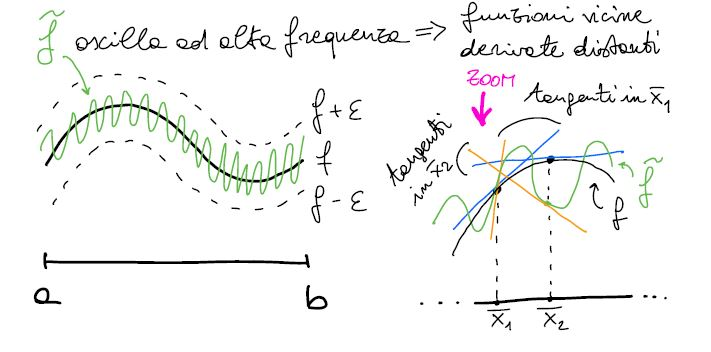
\includegraphics[scale=0.6]{calcolo55.JPG}
\end{center}
\textbf{\underline{FORMULE DI QUADRATURA}}\\
Passiamo ora ad introdurre il tema dell'\underline{integrazione numerica}, cioè degli algoritmi per il calcolo approssimato degli integrali.\\Ci sono 2 motivazioni per cercare algoritmi approssimati basati su un campionamento di $f$.\\La prima è che nelle applicazioni $f$ di solito non è nota in forma analitica ma sono noti solo dei valori campionati su un set di nodi in $[a,b]$; quello che di solito si può fare è infittire il campionamento.\\
Ma anche quando $f$ è nota analiticamente, non è detto che sia possibile calcolarne l'integrale analiticamente, utilizzando il teorema fondamentale del calcolo:
\begin{equation*}
    \int_a^b f(x)dx=F(b)-F(a)
\end{equation*}
dove $F$ è una primitiva di $f$, cioè $F'(x)=f(x)$; come noto, due primitive differiscono di una costante
\begin{equation*}
    \{F:F'=f\}=\{F=G+c,\,G'=f,\,c\in\mathbb{R}\}
\end{equation*}
dove $G$ è una primitiva fissata, ad esempio la funzione integrale
\begin{equation*}
    G(x) = \int_{a}^{x} f(t) dt, \ x \in [a,b]
\end{equation*}
Infatti ci sono funzioni esprimibili tramite funzioni elementari (cioè funzioni che si possono scrivere tramite somme e differenze, prodotti, divisioni, radicali e composizioni di: polinomi, funzioni razionali (rapporti di polinomi), funzioni trigonometriche (e inverse), esponenziali, logaritmi), le cui primitive \underline{non} sono esprimibili tramite funzioni elementari. \\
Questo accade con le primitive, mentre le derivate di funzioni esprimibili tramite funzioni elementari restano esprimibili tramite funzioni elementari. \\
Ad es., la primitiva (normalizzata) della gaussiana $f(x) = e^{-x^2}$, cioè la cosiddetta "error function"
\begin{equation*}
    erf(x) = \frac{2}{\sqrt{\pi}} \int_0^x e^{-t^2} dt, \ x \in \mathbb{R}
\end{equation*}
non è esprimibile tramite funzioni elementari (c'è una intera teoria dietro a questo risultato, che culmina nel "teorema di Liouville"), ma è di tale importanza nelle applicazioni che tutti i linguaggi di calcolo (ad es. il Matlab) la contengono come funzione predefinita, calcolata alla precisione di macchina (un altro esempio in cui la primitiva non è esprimibile elementarmente è $f(x) = \frac{\sin{x}}{x}$).\\
Un'idea semplice per il calcolo approssimato degli integrali è di sostituire all'integranda $f \in C[a,b]$ una funzione interpolante $f_n$ su $n+1$ nodi distinti $\left\{x_i\right\} \subset [a,b]$
\begin{equation*}
    f_n(x_i) = y_i = f(x_i), \quad 0 \leq i \leq n
\end{equation*}
Utilizzando i 2 tipi di interpolazione studiati nelle lezioni precedenti, si ottengono 2 famiglie di formule, dette FORMULE DI QUADRATURA, le cosiddette \underline{FORMULE ALGEBRICHE} (spesso chiamate anche "interpolatorie") per
\begin{equation*}
    f_n(x) = \inter_n(x)
\end{equation*}
cioè il polinomio interpolatore di grado $\leq n$, mentre per 
\begin{equation*}
    f_n(x) = \inter_s^c(x)
\end{equation*}
cioè la funzione polinomiale composta a tratti di grado locale $s$ (in questo caso come sappiamo $n$ deve essere multiplo di $s$), si ottengono le cosiddette \underline{FORMULE COMPOSTE}. \\
Per prima cosa facciamo vedere che entrambi i tipi di formule, diciamoli
\begin{equation*}
    I_n(f) = I(f_n) = \int_a^b f_n(x) dx
\end{equation*}
hanno la forma di somma pesata dei valori campionati
\begin{equation*}
    I_n(f) = \sum_{i=0}^n w_i f(x_i)
\end{equation*}
Infatti nel caso delle formule algebriche $I(f_n)=I(\inter_n)$ e ricordando la forma di Lagrange dell'interpolatore
\begin{equation*}
    \begin{split}
        I_n(f) = I(\inter_n) & = \int_a^b \inter_n(x) dx \\
        & = \int_a^b \left(\sum_{i=0}^n y_i l_i(x)\right) dx \\
        & = \sum_{i=0}^n \int_a^b y_i l_i(x) dx \\
        & = \sum_{i=0}^n w_i y_i \quad \text{con} \quad \overbrace{w_i}^{PESI} = \int_a^b l_i(x) dx, \quad 0 \leq i \leq n
    \end{split}
\end{equation*}
cioè i pesi sono gli integrali dei polinomi elementari di Lagrange (e quindi dipendono solo dai nodi). \\
Nel caso delle formule composte, ricordando che i nodi con $n=k\cdot s$ sono a pacchetti di $s+1$ con un nodo di raccordo
\begin{equation*}
    \begin{split}
        a = & x_0 < x_1 < \dotso < x_s \\
        & x_s < \dotso < x_ {2s} \\
        & \vdots \\
        & x_{(k-1)s} < \dotso < x_{ks} = x_n = b
    \end{split}
\end{equation*}
possiamo scrivere
\begin{equation*}
    \begin{split}
        I_n(f) = I(\inter_c^s) & = \int_a^b \inter_s^c(x) dx \\
        & = \sum_{j=1}^k \int_{x_{(j-1)s}}^{x_{js}} \inter_s^c(x) dx \\
        & = \sum_{j=1}^k \int_{x_{(j-1)s}}^{x_{js}} \inter_{s,j}(x) dx
    \end{split}
\end{equation*}
(dove $\inter_{s,j}$ è l'interpolazione locale di grado $\leq s$ sul tratto $[x_{(j-1)s},x_{js}]$ cioè $\inter_{s,j}(x)=\sum_{i=(j-1)s}^{js} y_i l_{i,j} (x)$, $i$-esimo pol. elementare relativo al pacchetto $x_{(j-1)s, \dotso , x_{js}}$)
\begin{equation*}
    \begin{split}
        & = \sum_{j=1}^k \int_{x_{(j-1)s}}^{x_{js}} \left(\sum_{i=(j-1)s}^{js} y_i l_{i,j}(x) \right) dx \\ 
        & = \sum_{j=1}^k \sum_{i=(j-1)s}^{js} y_i \int_{x_{(j-1)s}}^{x_{js}} l_{i,j}(x)dx \\
        & = \sum_{j=1}^k \sum_{i=(j-1)s}^{js} y_i w_{i,j}
    \end{split}
\end{equation*}
dove 
\[w_{i,j} = \int_{x_{(j-1)s}}^{x_{js}} \underset{\underset{\underset{\underset{\text{\underline{solo} dai nodi)}}{\text{(dipendono}}}{\textbf{PESI}}}{\uparrow}}{l_{i,j}(x)} , \quad (j-1)s \leq i \leq js \quad  1 \leq j \leq k\]
Ora, ciascun valore $y_i$ compare una volta tranne per i nodi di raccordo in cui compare 2 volte (quindi i 2 pesi corrispondenti vanno sommati).\\
Riarrangiando la doppia somma si arriva quindi a
\[
I_n (f) = I(\inter_s^c) = \sum_{i=0}^n w_i \cdot y_i
\]
dove $w_i = w_{i,j}$ per $(j-1) \cdot s < i < j \cdot s$
\[
w_i = w_{i,j} + w_{i,(j+1)}, \quad i=j \cdot s, \quad 1 \leq j \leq k-1
\]
Siccome il calcolo appena effettuato è formalmente piuttosto complicato, facciamo due esempi nel caso di nodi equispaziati, che danno luogo a due delle formule composte più usate.
\begin{enumerate}
    \item $s=1$: formula composta dei \underline{TRAPEZI} (generata dall'interpolazione lineare a tratti).
    \item $s=2$: formula composta delle \underline{PARABOLE} (generata dall'interpolazione quadratica a tratti).
\end{enumerate}
Vale la pena di mostrare subito l'interpretazione geometrica
\begin{center}
    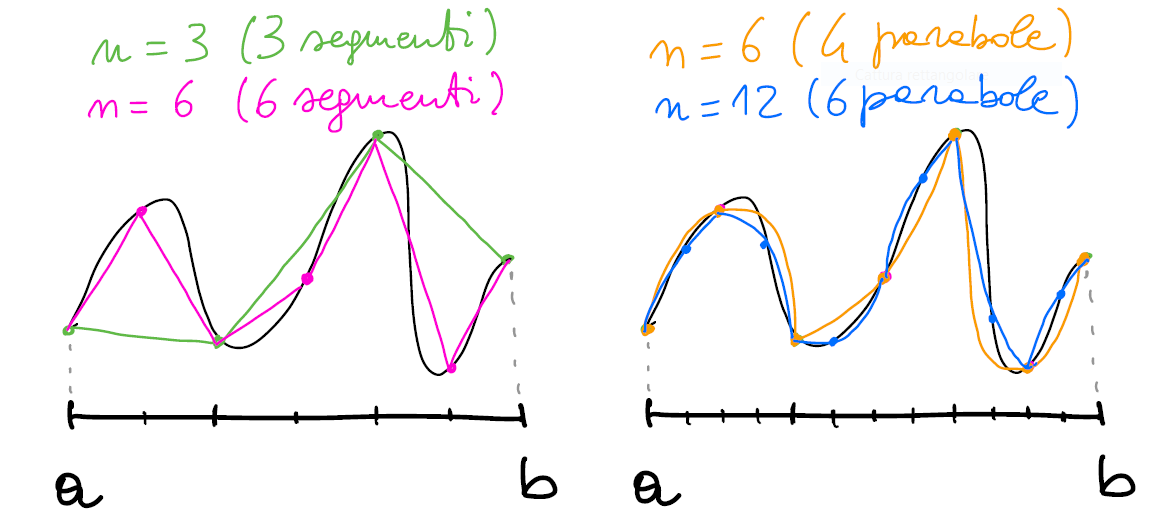
\includegraphics[width=0.7\textwidth]{pag17.png}
    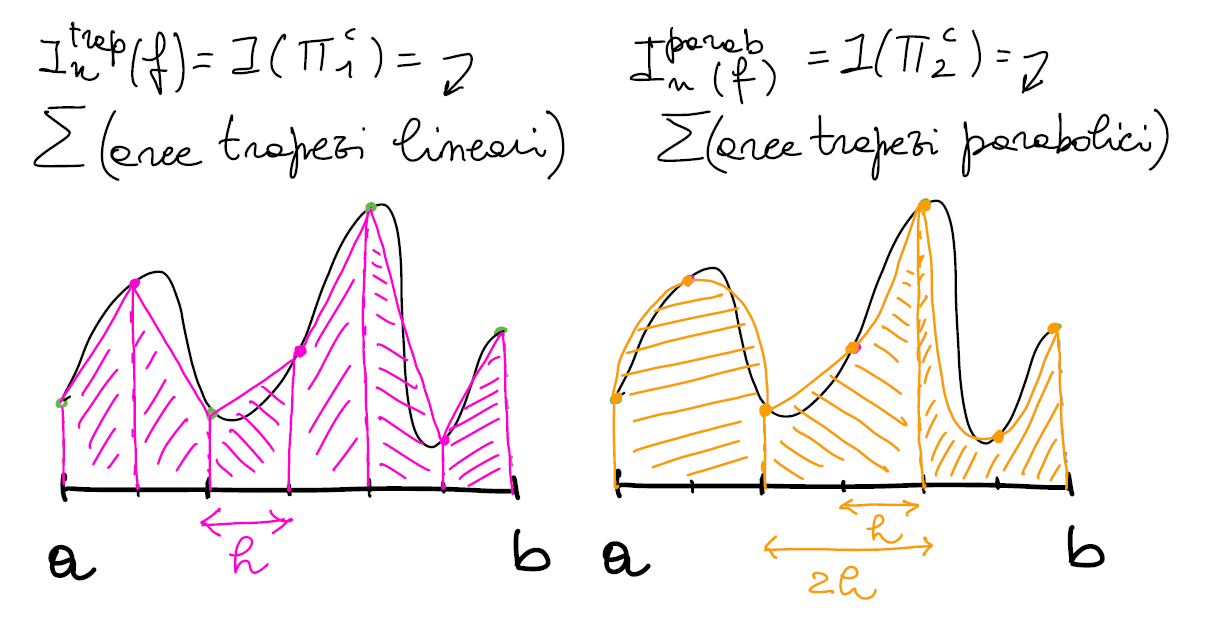
\includegraphics[width=0.7\textwidth]{pag18.png}
\end{center}
Per $s=1$ l'integrale $I(f)$ (cioè l'area che sta "sotto" la curva grafico di $f$) viene approssimata dalla somma delle aree dei trapezi lineari corrispondenti all'interpolante lineare a tratti.\\
Osservando che l'$i$-esimo trapezio ha altezza $h=(b-a)/n$ e basi $f(x_{i-1})$ e $f(x_i)$, $1 \leq i \leq n$, si ha area trapezio $i$-esimo $= \frac{h}{2} \cdot (f(x_{i-1}) + f(x_i))$ e quindi
\[
\begin{split}
    I_n^{trap} (f) & = I(\inter_1^c) \\
    & = \int_a^b \inter_1^c (x) dx \\
    & = \sum (\text{aree trapezi}) \\
    & = \overbrace{\frac{h}{2} \cdot (f(x_0) + f(x_1))}^{\text{area trapezio 1}} + \overbrace{\frac{h}{2} \cdot (f(x_1) + f(x_2))}^{\text{area trapezio 2}} + \dotso + \\
    & + \underbrace{\frac{h}{2} \cdot (f(x_{n-2}) + f(x_{n-1}))}_{\text{area trapezio (n-1)-esimo}} + \underbrace{\frac{h}{2} \cdot (f(x_{n-1}) + f(x_n))}_{\text{area trapezio n-esimo}} \\ 
    & =\frac{h}{2} (f(x_0) + f(x_n)) + \sum_{i=1}^{n-1} h \cdot f(x_i)
\end{split}
\]
(perché ogni nodo interno $x_i$, $1 \leq i \leq n-1$, compare in 2 trapezi consecutivi, cioè la FORMULA DEI TRAPEZI)
\[
I_n (f) = \sum_{i=0}^n w_i \cdot f(x_i), \ \text{con} \ w_i =
\begin{cases}
\frac{h}{2}, \quad i=0,n \\
h, \quad 1 \le i \le n-1
\end{cases}
\]
Nel caso $s=2$, integrando la funzione quadratica a tratti $\inter_2^c$ si ottiene (dimostrazione non richiesta) la FORMULA DELLE PARABOLE (detta anche formula di Simpson).
\[
I_n^{parab} (f) = I \left(\inter_2^c\right) = \sum (\text{aree trapezi parabolici}) \\
= \sum_{i=0}^n w_i \cdot f(x_i), \ \text{con} \ w_i = 
\begin{cases}
h/3,  \quad i=0, \, n \text { pari}\\
2h/3, \quad i \ \text{dispari}\\
4h/3, \quad i \ \text{pari} \ 2 \leq i \leq n-2
\end{cases}
\]
La formula si ottiene calcolando l'integrale di una interpolante di grado 2 su $[\alpha, \beta]$ costruita con i valori $f(\alpha), \ f(\beta), \ f((\alpha+\beta)/2)$
\[
\int_\alpha^\beta \inter_2 (x) dx = \frac{h}{3} \cdot f(\alpha) + \frac{4}{3} \cdot h \cdot f\left(\frac{\alpha + \beta}{2}\right) + \frac{h}{3} \cdot f(\beta)
\]
\begin{center}
    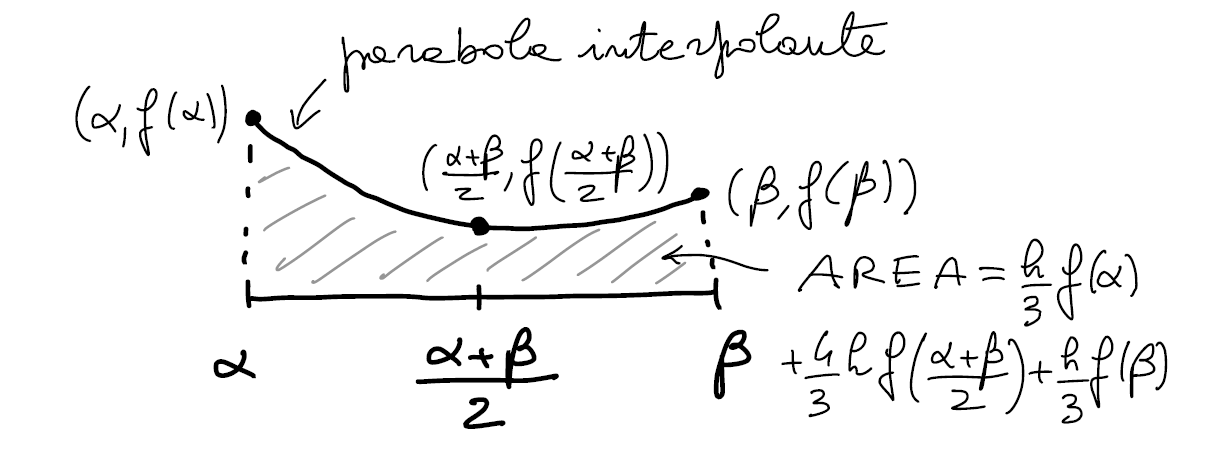
\includegraphics[width=0.8\textwidth]{pag21.png}
\end{center}
Si osservi che entrambe le formule hanno \underline{pesi positivi}.\\
In realtà, non è affatto sorprendente che le formule di approssimazione siano somme pesate, si pensi alla definizione stessa di integrale come limite delle somme integrali superiori e inferiori su partizioni.\\
Il punto però è trovare somme "furbe", che garantiscono una buona approssimazione con "pochi" termini (sfruttando le proprietà di $f$).\\\\
\fbox{\textbf{CONVERGENZA}}\\
Nell'analisi di convergenza la domanda è: per quali distribuzioni di nodi e per quali integrande $f$ si ha
\[
\lim_{n \to \infty} I_n (f) = I(f) ?
\]
dove $I_n(f) = \sum_{i=0}^n w_i \cdot y_i$, $y_i = f(x_i)$, è una successione di formule di quadratura.\\
Visto che abbiamo costruito le formule usando una funzione interpolante
\[
f_n(x): f_n(x_i) = f(x_i), \ \ 0 \le i \le n
\]
cioè $I_n(f) = I(f_n)$\\
Ci viene in aiuto la stima fondamentale ricavata a inizio lezione (ponendo $\tilde{f} = f_n$)
\[
\begin{split}
\abs{I(f) - I_n(f)} & = \abs{I(f) - I(f_n)} \\
& = \abs{I(f - f_n)} \\
& \le I(\abs{f - f_n}) \\
& \le (b-a) \cdot dist(f, f_n)
\end{split}
\]
Se $dist(f, f_n) \to 0, \ n \to \infty$ (convergenza dell'interpolazione) avremo convergenza anche per le formule di quadratura; se invece $dist(f, f_n)$ non va a 0 (o addirittura diverge) ci aspettiamo problemi
di convergenza anche per le formule di quadratura.\\\\
\textbf{Formule algebriche}\\
In questo caso $f_n=\inter_n$ quindi 
\begin{equation*}
    |I(f)-I_n(f)|\leq(b-a)dist(f,\inter_n)
\end{equation*}
Con le formule ottenute integrando $\inter_n^{eq}$ (il polinomio interpolatore su nodi equispaziati), dette formule di Newton-Cotes, ci aspettiamo problemi perchè sappiamo che $dist(f,\inter_n^{eq})$ può divergere anche per funzioni molto regolari (vedi esempio di Runge).\\
Dalle stime dell'errore di interpolazione sappiamo che tali formule possono convergere per particolari funzioni, ad esempio per funzioni $C^{\infty}$ con derivate equilimitate (ad es. $f(x)=e^x$), ma si può dimostrare (non lo faremo) che in generale le formule di Newton-Cotes (\underline{algebriche} su nodi \underline{equispaziati non sono convergenti}).\\ Invece se le formule sono ottenute interpretando il polinomio interpolatore su nodi di tipo \underline{Chebyshev} abbiamo che \\
\begin{equation*}
    dist(f,\inter_n^{Cheb})\leq c_k\frac{log(n)}{n^k}
\end{equation*}
per $f\in C^k[a,b]$, e quindi tali formule sono sicuramente \underline{convergenti} per $f\in C^k[a,b]$, \ $k>0$.\\\\
\textbf{Formule composte}\\
La situazione cambia completamente con le formule composte, ottenute come $I_n(f)=I(\inter_s^c)$, con $n$ multiplo di $s$.\\Infatti per tali formule $s$ è fissato e
\begin{equation*}
\begin{split}
    |I(f)-I_n(f)|\leq(b-a)\cdot dist(f,\inter_s^c)\leq(b-a)k_s\cdot h^{s+1} \  \  \  \  \  \text{se} \ f\in C^{s+1}[a,b]
\end{split}
\end{equation*}
con $h = max \ \Delta x_i$.\\
Quindi per qualsiasi distribuzione di nodi per cui $h\rightarrow0$ (in particolare per i nodi equispaziati, $h=\frac{b-a}{n}$) se $f\in C^{s+1}[a,b]$ le corrispondenti formule sono \underline{sempre convergenti} con un errore proporzionale a $h^{s+1}$.\\Ad esempio per $f\in C^2$ la formula dei trapezi ha un errore di ordine $h^2$ e la formula della parabola ha un errore di ordine $h^3$ per $f\in C^3$.\\
Addirittura, nel caso di nodi equispaziati si può far vedere che la formula della parabola ha un errore di ordine $h^4$ se $f\in C^4$ (la dimostrazione, che non facciamo, non si basa sulla stima scritta sopra che darebbe comunque ordine $h^3$, ma su conti specifici che usano la simmetria locale dei nodi).\\\\
\textbf{STABILITA'}\\
L'analisi di stabilità parte dall'osservazione, già fatta per l'interpolazione, che in pratica
nelle applicazioni i valori campionati $y_i=f(x_i)$, $0\leq i\leq n$, non sono mai noti esattamente, ma abbiamo invece a disposizione dei valori perturbati $\tilde{y}_i\approx y_i$, dove assumiamo di avere una stima 
\begin{equation*}
    \underset{i}{max}|y_i-\tilde{y}_i|\leq \varepsilon
\end{equation*}
La domanda diventa: qual è la "risposta" della formula di quadratura agli errori sui dati? Cioè come si può stimare in funzione di $\varepsilon|I_n(f)-\tilde{I}_n(f)|$, dove $\tilde{I_n}(f)=\sum_{i=0}^nw_i\tilde{y}_i$?\\
La stima è semplice:
\[\begin{split}
    \abs{I_n(f) - \Tilde{I}_n(f)} & = \abs*{\sum_i w_i y_i - \sum_i w_i \Tilde{y}_i} \\
    & = \abs*{\sum_i w_i( y_i - \Tilde{y}_i)} \\
    \text{dis. triangolare} \to & \le \sum_i \abs*{w_i} \underbrace{\abs*{y_i - \Tilde{y}_i}}_{\le \varepsilon} \\
    & \le \sum_i \abs*{w_i} \cdot \varepsilon \\
    & = \varepsilon S_n, \quad S_n = \sum_{i=0}^n \abs*{w_i}
\end{split}\]
Cioè si vede che il ruolo giocato dalla costante di Lebesgue nell'interpolazione polinomiale, nelle formule di quadratura è giocato dalla quantità
\[S_n = \sum_{i=0}^n \abs*{w_i}\]
che modula la risposta agli errori.\\
Bene, avremo che le formule di quadratura sono \underline{stabili} (per $n \to \infty$) se $S_n$ è \underline{limitata}, cioè
\[\exists\, k > 0 : S_n \le k \quad \forall n\]
(Attenzione: $S_n$ \underline{non} è la somma parziale di una serie, perché cambiando $n$ cambiano in generale i nodi, $\{x_i\} = \{x_i(n)\}$, e i pesi $\{w_i\} = \{w_i(n)\}$ che dipendono (solo) dai nodi). \\
È facile vedere che le formule di quadratura algebriche e composte con PESI POSITIVI sono STABILI.\\
Infatti in tal caso:
\[S_n = \sum_{i=0}^n \abs*{w_i} = \sum_{i=0}^n w_i = \sum_{i=0}^n 1 \cdot w_i = \int_a^b 1 \cdot dx = b - a\]
cioè $S_n = b-a \quad \forall n$ (non solo è limitata, è addirittura costante).\\
Perché $\sum_i w_i = \sum_i 1 \cdot w_i = \int_a^b 1 \cdot dx$?\\
La prima uguaglianza dice che è come se stessimo applicando la formula alla funzione costante $f=1$; la seconda viene dal fatto
che sia le formule algebriche che le formule composte sono "esatte", cioè fanno errore zero, sulle funzioni costanti (che sono polinomi di grado 0).\\
Infatti l'interpolazione con un unico polinomio $\inter_n$ fa errore zero se $f \in \mathbb{P}$ e $deg(f) \le n$ ($deg(f)$ significa $grado(f)$), mentre l'interpolazione a tratti fa errore zero se $f \in \mathbb{P}$ e $deg(f) \le s$ (in entrambi i casi per l'unicità della funzione interpolante).\\
Purtroppo non tutte le formule di quadratura hanno pesi $>0$.\\
In particolare, i pesi delle formule di \underline{Newton - Cotes} (algebriche su nodi equispaziati) sono positivi per $n \le 7$, mentre per $n>7$ cominciano ad apparire pesi negativi e il modulo dei pesi cresce in modo tale che $S_n$ diverge esponenzialmente (rendendo tali formule molto instabili, quindi in pratica inutilizzabili anche per le speciali funzioni, ad es. $f(x) = e^x, \ sin(x), \ cos(x)$, per cui sarebbero teoricamente convergenti).\\
Invece proprio per quanto appena detto le formule composte di grado $s \le 7$ sono a pesi positivi e quindi stabili (localmente sono formule di Newton - Cotes di grado fissato, le più usate sono quelle con $s=1$ (trapezi), $s=2$ (parabole), $s=3$ (cubiche)).\\
Per quanto riguarda le formule algebriche, si può dimostrare (ma la dimostrazione è difficile) che quelle ottenute da nodi tipo \underline{Chebyshev} hanno \underline{pesi positivi} e quindi sono \underline{stabili} oltre che \underline{convergenti}.\\
Riassumendo:
\[
\begin{split}
\abs{I(f) - \tilde{I_n}(f)} & = \abs{I(f) - I_n(f) + I_n (f) - \tilde{I_n}(f)} \\
& \le \underbrace{\abs{I(f) - I_n (f)}}_{\text{CONVERGENZA?}} + \underbrace{\abs{I_n (f) - \tilde{I}_n (f)}}_{\text{STABILITÀ?}}
\end{split}
\]
Ad esempio per le formule di "tipo Chebyshev" con $f \in C^k [a,b], \ k > 0$
\[
\abs{I(f) - \tilde{I}_n^{cheb}(f)} \le \underbrace{(b-a) C^k \frac{log(n)}{n^k}}_{\to 0, \ n \to \infty} + \underbrace{(b-a)\varepsilon}_{\text{STABILI}}
\]
mentre per le formule composte con $s \le 7$ (trapezi, parabole, cubiche, $\dotso$)
\[
\abs{I(f) - \tilde{I}_n(f)} \le \underbrace{(b-a)k_s h^{s+1}}_{\to 0, \ h \to 0} + \underbrace{(b-a)\varepsilon}_{\text{STABILI}}
\]
Concludiamo dicendo che abbiamo visto solo alcuni aspetti introduttivi e parziali della vasta teoria dell'integrazione numerica.\\
Ad esempio la costruzione di formule di quadratura si può estendere a integrali generalizzati del tipo
\[
I_w (f) = \int_a^b f(x) \cdot w(x) dx
\]
con $f \in C[a,b]$ e $w$ "funzione peso" positiva, continua e integrabile in $(a,b)$ (ma non necessariamente limitata, ad esempio $w(x) = (1-x^2)^{-1/2}, \ [a,b] = [1,1]$).\\
In questo contesto ci sono ad esempio le cosiddette formule gaussiane, che sono formule algebriche a pesi positivi, costruibili per qualsiasi funzione peso $w$ e convergenti per qualsiasi $f \in C [a,b]$.\\
In effetti la teoria della convergenza è molto più fine di quella che abbiamo tracciato con la stima fondamentale
\[
\abs{I(f) - I(f_n)} \le (b-a) \cdot dist(f, f_n)
\]
Ad esempio, si può dimostrare che le \underline{formule a pesi positivi} non solo sono \underline{stabili} (come
abbiamo visto) ma sono anche \underline{convergenti} all'integrale di \underline{qualsiasi funzione continua} (la teoria corrispondente culmina nel "teorema di Polya - Stelkov").


\end{document}
